%-----------------------------------------------------------------------
% 
%-----------------------------------------------------------------------
%
%     
%
%
%%%%%%%%%%%%%%%%%%%%%%%%%%%%%%%%%%%%%%%%%%%%%%%%%%%%%%%%%%%%%%%%%%%%%%%%


\documentclass[twoside]{article}
\usepackage{amsmath,amsthm,amssymb,verbatim}

%     If your article includes graphics, uncomment this command.
\usepackage{graphicx}

%     If the article includes commutative diagrams, ...
%\usepackage[cmtip,all]{xy}

\usepackage{url}

\usepackage{fancyhdr}
\pagestyle{fancy}

\def\blfootnote{\xdef\@thefnmark{}\@footnotetext} 
\long\def\symbolfootnote[#1]#2{\begingroup%
\def\thefootnote{\fnsymbol{footnote}}\footnote[#1]{#2}\endgroup} 

	\addtolength{\oddsidemargin}{1cm}
	\addtolength{\evensidemargin}{-1cm}

\setcounter{page}{1}

\begin{document}

%     If you need symbols beyond the basic set, uncomment this command.
%\usepackage{amssymb}


\newtheorem{theorem}{Theorem}[section]
\newtheorem{lemma}[theorem]{Lemma}

\theoremstyle{definition}
\newtheorem{definition}[theorem]{Definition}
\newtheorem{example}[theorem]{Example}
\newtheorem{xca}[theorem]{Exercise}

\theoremstyle{remark}
\newtheorem{remark}[theorem]{Remark}

\numberwithin{equation}{section}


\date{}
\lhead[]{}
\chead[\underline{New Symmetry Properties }]{\it{O. Shanker}}
\rhead[]{}

% \title[short text for running head]{full title}
\title{\bf{New Symmetry Properties of Value Distribution of Hardy $Z$ Function}}

\maketitle


%    author one information
% \author[short version for running head]{name for top of paper}
\author{{\textbf{O. Shanker}},}
\thanks{ Mountain View, CA 94041, U. S. A. email: oshanker@gmail.com}

\thispagestyle{fancy}

%    Abstract is required.
\begin{abstract}
The human mind is attracted by symmetry. Many objects in nature exhibit symmetry.
Even more remarkable are the symmetries exhibited in the basic laws of the 
universe. In this work we discuss a new hitherto unknown symmetry in the value
distribution of the Hardy $Z$ function at discrete points. This is significant because symmetry properties
are fundamental aspects of a system. It should be noted that the Hardy $Z$ function is closely
related to the famed Riemann zeta function.

\end{abstract}
{\textbf {Keywords}:} Riemann zeta, Value Distribution, Symmetry, Hardy's function
{\textbf {Mathematics Subject Classification (MSC)}:} 11M06, 11-04.


\symbolfootnote[0]{\bf{* }}


\section{Introduction}

The symmetries exhibited by a system are fundamental aspects of the system. Thus, it is very exciting when we find a new symmetry in studying any phenomenon. In this work, we present a symmetry property and an anti-symmetry property for the value
distribution of the Hardy $Z$ function at discrete points.

Our symmetries will be expressed in terms of Gram points~\cite{Gram 1903}. Gram points and  Gram intervals are well known topics of study in the literature pertaining to the Riemann Hypothesis. For completeness we present the definitions in Section~\ref{sec2}.


We were motivated to study the topic because of the result of Titchmarsh~\cite{Titchmarsh 1934} . He showed that the mean value of the Hardy function was 2 at even Gram points and -2 at odd Gram points. We wondered if the property could be generalized to the statement that the underlying distributions were themselves anti-symmetric. Ref.~\cite{Shanker 2018a} studied empirically the distribution of $Z(t)$ values at Gram points and showed  that this was indeed the case. We further wondered if  the property could be extended to other discrete points on the critical axis. The new symmetries we discovered as a result of the investigation  are that the  value
distribution of the Hardy $Z$ function at discrete points is anti-symmetrical for reflections around the mid-points of the Gram intervals (Eq.~\ref{eq:antisym}) and symmetrical for reflections around the Gram points(Eq.~\ref{eq:sym}). We tested the symmetry properties for samples spanning $16$ orders of magnitude.

\begin{table}
\centering \(\begin{array}{ccccccc}
\hline
 \phi &     Min.   &  \multicolumn{2}{c}  {Median }   &   Mean   &  \multicolumn{2}{c}  {Max.} \\
  \cline{3-7}  
 &              & Quantile   &      x      &              & Quantile.    &  y \\
\hline
0 &-69 &0.1134 &0.8517 &2.0001 &2.5403 &165  \\
\pi/4 &-97 &-0.1352 &0.5916 &1.4143 &2.1226 &159 \\
\pi/2 &-121 &-1.082 &0.0017 &0.0001 &1.089 &137 \\
3\pi/4&-148 &-2.1121 &-0.5852 &-1.4141 &0.1364 &103 \\
\pi &-161 &-2.5277 &-0.8467 &-1.9999 &-0.1122 &69 \\
5\pi/4 &-153 &-2.1045 &-0.5891 &-1.4141 &0.1365 &105 \\
3\pi/2 &-129 &-1.083 &-0.001 &0.0001 &1.084 &138 \\
7\pi/4 &-93 &-0.1336 &0.5883 &1.4143 &2.1077 &160 \\
\hline
\end{array}\)
\caption{Quantiles and mean for  $Z(t)$ when $\phi$ values are multiples of $\pi/4$.} 
\label{tab:multicolumn}
\end{table}

\begin{figure*}
\centering
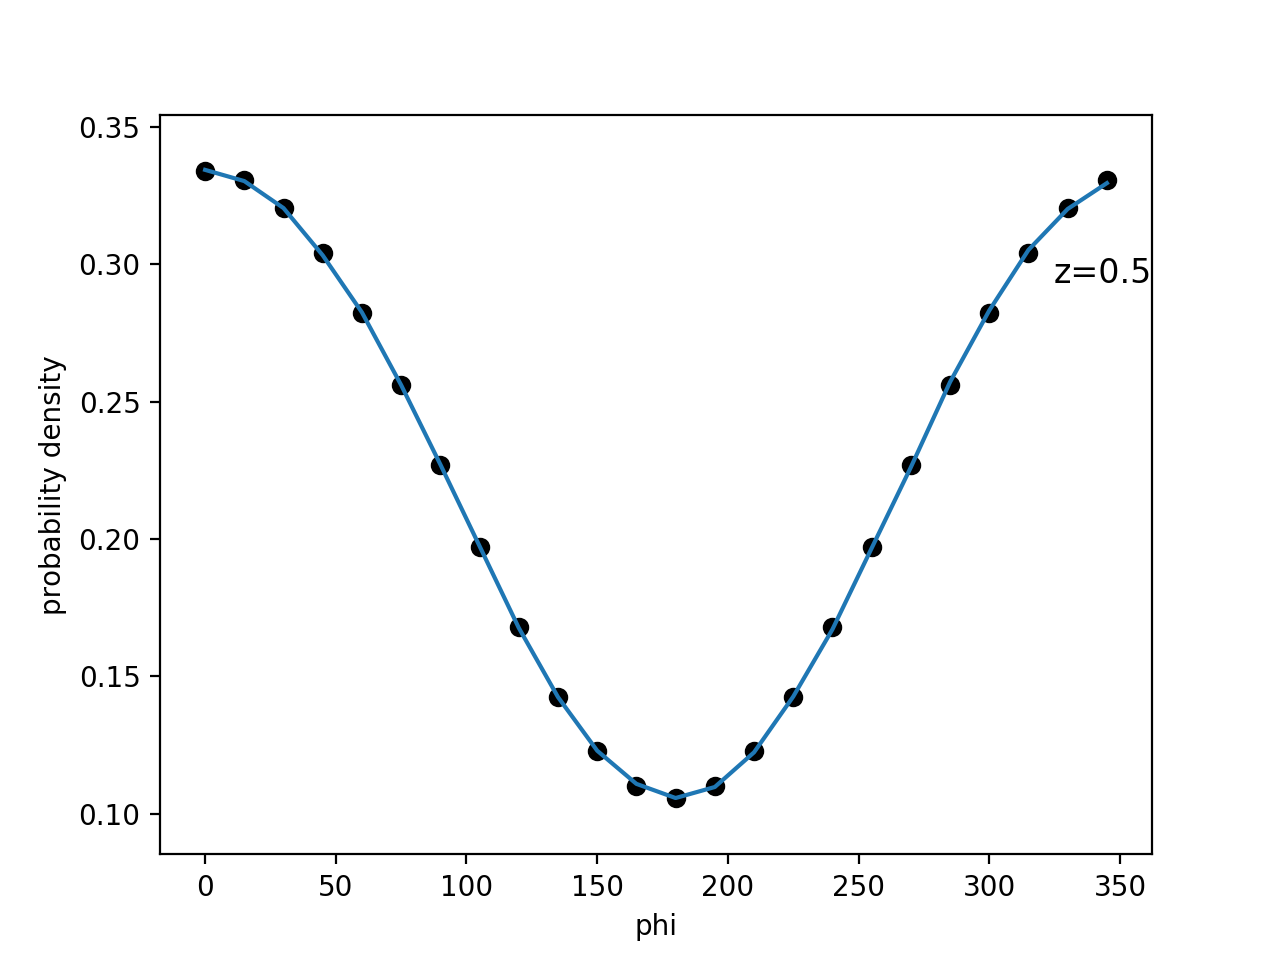
\includegraphics[width=0.8\textwidth]{z05.png}
\caption[]{ 
 Distribution of zeta values at $\phi = \pi/2$.
  }
\vspace{1mm}
\label{pi2}
\end{figure*}

\section{\label{sec2}Notation for the Riemann zeta function}

In this section we  establish the required notation for the 
Riemann Zeta Function. 
For $\mathrm{Re} (s) > 1$ the Riemann Zeta function is defined as
\begin{equation}
\zeta ( s ) \, = \, \sum^{\infty}_{n = 1} \; n^{-s} \, = \, \prod_{p \in primes} \;
\left( 1 - p^{-s} \right)^{-1}.
\label{eqRie}
\end{equation}
 $\zeta ( s )$ can be continued to
the complex plane. Riemann's hypothesis, that the non-trivial zeros of $\zeta ( s )$ lie on the 
critical axis $1/2+it$, is probably the most famous unsolved problem in mathematics.
The mean spacing $\delta$ of the zeros  at large height $T$ is $\delta = 2\pi(\ln (T/2\pi))^{-1}$. 
For numerical studies of the Riemann hypothesis one defines Hardy's function
\begin{equation}
Z(t)=exp(i\theta(t))\zeta(1/2 +it) 
\label{eq:hardy}
\end{equation}
where 
\begin{equation}
\theta(t) = arg (\pi^{it/2} \Gamma(\frac{1}{4} + \frac{it}{2})). 
\label{eq:theta}
\end{equation}
The argument in Eq.~\ref{eq:theta} is defined by continuous variation of $t$ starting with the value $0$ at $t = 0$.
$Z(t)$ is real valued for real $t$,
and we have $|Z(t)| = |\zeta(1/2+it)|$. Thus the zeros of $Z(t)$ are the imaginary part of the zeros 
of $\zeta(s)$ which lie on the critical line.  

Gram points play an important role in the the theory because many of the zeros are separated by them.  When $t \ge 7$, the $\theta$ function Eq.(\ref{eq:theta}) is monotonic increasing. 
For $n \ge -1$, the $n$-th Gram point $g_n$ is defined as the unique solution $> 7$ to
$\theta (g_n) = n\pi$. A Gram interval is the interval $G_n = [g_n,g_{n+1})$.
 In analogy with Gram points, we can associate an angle $\phi$ with a point $t$ on the critical axis as follows:
\begin{definition}\label{phi}
For $t \ge 7$, $t$ is said to be a generalized Gram point with value $\phi$  if
$\theta (t) = 2k\pi + \phi$, where $0 \le \phi < 2\pi$.
\end{definition}


\section{\label{sec3}Quantiles}
In this section we present our numerical studies. The results provide very good evidence for two new symmetry properties (see also \cite{Shanker 2018b}).
We first give a brief overview of the current state of the literature on the subject. We then present the distribution for $T=10^{12}$, followed by the distribution for $T=10^{28}$. We are interested in how the symmetry properties behave when we span a large range of height $T$.

The sample space for our study is the interval along the critical axis specified by $(T_1, T_2)$. While empirical studies necessarily use large but finite  $T_1, T_2$, we are interested in the limit 
$T_1 \rightarrow \infty, T_2 \rightarrow \infty,  T_2-T_1 \rightarrow \infty,$ however
\begin{equation}
T_2 - T_1  \ll T_1. 
\label{eq:interval}
\end{equation}
Because of Equation \ref{eq:interval}, we can consider  $\ln (t)$  to be effectively constant over  the interval.
We use
$10^6$ Gram intervals in our samples. We studied  two samples, $T_1=10^{12}$ and  $T_1=10^{28}$. We chose these samples because  Ref~\cite{hiary 2010} has evaluated all the zeros in these ranges. We consider all $Z(t)$ values for a given $\phi$ in the sample space.

We will present the symmetry properties in terms of the quantiles~\cite{Feller 1971} for the sample space. This is because for any sample space the quantiles are well defined and always exist. We recall that in statistics, given a fraction $f$ between $0$ and $1$, the quantile $q_f$ is the value such that fraction $f$  of the sample population is at or below $q_f$. For example, $q_{0.5}$ is the median of the sample.
For $f$ very close to $0$ or $1$, in the limiting case $q_f$ will diverge. However we will assume that there is a range of $f$ for which well-defined limits exist. If necessary we can normalize the $Z$ values by some power of $\ln(T/2\pi)$ without affecting the symmetry properties. Since the standard deviation is known to be $sqrt(\ln(T/2\pi))$~\cite{Shanker 2018b}, normalizing $Z$ by this factor will make $q_f$ finite for finite $f$. Certainly, for our two samples separated by several orders of magnitude, we find that the quantile distribution changes very little. 

The anti-symmetry relation is
\begin{equation}
q_{f}(\phi) = -q_{1-f}(\pi-\phi).
\label{eq:antisym}
\end{equation}
Equation~\ref{eq:antisym}  is a generalization of the result in Ref.~\cite{Shanker 2018a} for the anti-symmetry of the distribution of $Z(t)$ at even and odd Gram points. The  symmetry condition is
\begin{equation}
q_{f}(\phi) = q_{f}(2\pi-\phi).
\label{eq:sym}
\end{equation}


We briefly mention other studies of the value distribution of the Riemann zeta function and the closely related Hardy's function~\cite{Hardy 1918}.  Ivi\'c's monograph~\cite{Ivic 2013} has a comprehensive survey of  the field.
Selberg in unpublished work showed that at large $t$ $\log (\zeta(\frac{1}{2} + it))$ is approximately normally distributed with a standard deviation of order $\sqrt{log~log~t}$ (see Ref.~\cite{Hejhal}). He showed a 
similar result~\cite{Selberg 1989, Selberg 1991} for $\log (|Z(t)|)$. Laurincikas~\cite{Laurincikas}  used probabilistic number theory to prove various results about the distribution of the Riemann zeta function.

Regarding the value distribution at specific points along the Gram interval, Titchmarsh~\cite{Titchmarsh 1934} and Kalpokas and Steuding~\cite{kalpokas 2009} present results pertaining to the
mean value of the Riemann zeta function. Lester's~\cite{Lester 2013} Ph. D. thesis also considers the distribution of $\log (|\zeta(\frac{1}{2} + it)|)$  for specific points along the Gram interval.  
The question of the values of Hardy's $Z$-function at a discrete sequence of points on the critical axis is quite interesting. The above references give some results in this direction that can be proved rigorously. At the same time, the present state of Riemann zeta function theory gives limited information about the value distribution of $Z(t)$ at discrete sequences of points. Possibly, these analogues could differ significantly from the continuous case. To investigate the question we perform a numerical study of the value distribution of Hardy's $Z$-function at discrete points. 


\subsection{\label{E12}Quantiles for $Z(t)$ at $T=10^{12}$}


\begin{table}
\centering \(\begin{array}{cccccccccccc}

\hline
0&\pi/6 &\pi/3 &\pi/2 &2\pi/3 &5\pi/6 &\pi &7\pi/6 &4\pi/3 &3\pi/2 &5\pi/3 &11\pi/6 \\
2.000 &1.732 &1.000 &0.000 &-1.000 &-1.732 &-2.000 &-1.732 &-1.000 &0.000 &1.000 &1.732 \\
4.998&5.002&5.004&5.004&5.000&4.996&4.991&4.987&4.985&4.986&4.989&4.993 \\
\hline
\end{array}\)
\caption{Mean    $Z(t)$ and Standard Deviation at $T=10^{12}$. Row 1: $\phi$, Row 2: mean~$Z$, Row 3: Standard Deviation}
\label{tab:mean12}
\end{table}

\begin{table}
\centering \(\begin{array}{cccccccccccc}
\hline
\phi&0.1&0.2&0.25&0.3&0.4&0.5&0.6&0.7&0.75&0.8&0.9 \\
\hline
0&-0.687&-0.011&0.113&0.234&0.506&0.852&1.324&2.031&2.54&3.229&5.876\\
\pi/6 &-1.055&-0.161&0.017&0.138&0.401&0.732&1.188&1.865&2.352&3.008&5.577\\
\pi/3 &-2.068&-0.709&-0.388&-0.164&0.123&0.411&0.801&1.39&1.815&2.4&4.688\\
\pi/2 &-3.415&-1.543&-1.082&-0.75&-0.297&0.002&0.299&0.753&1.089&1.555&3.415\\
2\pi/3 &-4.693&-2.391&-1.81&-1.382&-0.795&-0.405&-0.119&0.165&0.39&0.713&2.068\\
5\pi/6 &-5.586&-3.006&-2.338&-1.852&-1.178&-0.726&-0.396&-0.137&-0.016&0.162&1.051\\
\pi &-5.9&-3.218&-2.528&-2.024&-1.319&-0.847&-0.503&-0.231&-0.112&0.012&0.687\\
7\pi/6 &-5.569&-2.995&-2.334&-1.851&-1.182&-0.729&-0.399&-0.137&-0.016&0.163&1.048\\
4\pi/3 &-4.674&-2.387&-1.803&-1.379&-0.799&-0.41&-0.123&0.166&0.388&0.712&2.066\\
3\pi/2 &-3.407&-1.543&-1.083&-0.75&-0.296&-0.001&0.297&0.751&1.084&1.549&3.403\\
5\pi/3 &-2.061&-0.705&-0.386&-0.164&0.122&0.409&0.797&1.384&1.81&2.391&4.67\\
11\pi/6 &-1.037&-0.159&0.018&0.14&0.4&0.732&1.183&1.851&2.339&3.004&5.56\\

\hline
\end{array}\)
\caption{Quantiles  for  $Z(t)$ at $T=10^{12}$.}
\label{tab:quantiles12}
\end{table}


\begin{table}
\centering \(\begin{array}{cccccccccccc}
\hline
$f$&0.1&0.2&0.25&0.3&0.4&0.5&0.6&0.7&0.75&0.8&0.9\\
\hline
intercept&-3.346&-1.569&-1.134&-0.817&-0.360&0.002&0.362&0.821&1.139&1.575&3.342\\
slope&1.307&0.817&0.678&0.577&0.457&0.420&0.457&0.578&0.681&0.819&1.302\\
R^2&0.999&0.999&0.997&0.995&0.996&1.000&0.996&0.995&0.997&0.999&0.999\\
\hline
\end{array}\)
\caption{Linear fit of quantile $q_f$ to $2\cos(\phi)$ at $T=10^{12}$.}
\label{tab:fit12}
\end{table}

\subsubsection{\label{numerics}Numerical evaluation}

Hardy's function $Z(t)$  is evaluated using the Riemann$-$Siegel series
\begin{equation}
Z(t) = 2\sum^{m}_{n=1}\frac{\cos(\theta(t) - t \ln (n))}{\sqrt{n}} + R(t), 
\label{eq:RS}
\end{equation}
where $m$ is the integer part of $\sqrt{t/(2\pi)}$. $R(t)$ is a small remainder
term which can be evaluated to the desired level of accuracy. We used the techniques in Refs.~\cite{Odlyzko 1992,hiary,gourdon} 
to efficiently evaluate the zeta function at large $t$. To evaluate  $Z(t)$  at several points in the Gram interval, we have to use band limited function interpolation~\cite{Jerri 1977}. We evaluate the coefficients in the series for band limited function interpolation at the Gram points, and use the series to evaluate $Z(t)$ at other points in the Gram interval. The most important 
source for loss of accuracy at large heights is the cancellation between
large numbers that occur in the arguments of the $\cos$ terms in Eq.~(\ref{eq:RS}). We 
use a high precision module to evaluate the arguments. The rest of the calculation
is done using regular double precision accuracy. The  zeros from Ref~\cite{hiary 2010} were used to check the accuracy of our zeta function calculations. Our evaluations of $Z(t)$ at $T=10^{12}$ are accurate to better than $10^{-6}$. 

\subsubsection{\label{discusssionE12}Results and symmetries}

Table~\ref{tab:mean12} shows the mean value for $Z(T)$ and the standard deviation at $12$ equally spaced values of $\phi$ at $T=10^{12}$. The mean value is known from theory to be $2\cos(\phi)$, and the standard deviation is known to be $sqrt(\ln(T/2\pi))$~\cite{Shanker 2018b}. The table verifies this result to better than one part in a thousand. Table~\ref{tab:quantiles12} shows the quantiles for $Z(T)$. Eq.~\ref{eq:antisym} can be verified, for example, by noting that $q_f$ in Table~\ref{tab:quantiles12}
for $\phi=\pi/6$ and $f=0.25$ is $0.017$, while it is $-0.016$ for $\phi=5\pi/6$ and $f=0.75$. Eq.~\ref{eq:sym} can be verified, for example, by noting that $q_f$ is $0.018$ for $\phi=11\pi/6$ and $f=0.25$.

We found that there is a linear dependence of the quantiles on $\cos(\phi)$. Table~\ref{tab:fit12} shows the intercept and slope when $q_f$ for any $f$ is fitted to
$2\cos(\phi))$. The observation of this relation itself verifies the symmetry condition Eq.~\ref{eq:sym} (i.e., there is no dependence on $\sin(\phi)$). The anti-symmetry condition Eq.~\ref{eq:antisym} implies that the intercept is anti-symmetric for reflection around $f=0.5$, while the slope is symmetric for such a reflection. This can be verified from the table. Table~\ref{tab:fit12} makes the symmetry and anti-symmetry relations stand out clearly.  It must be pointed out that Eq.~\ref{eq:antisym} and Eq.~\ref{eq:sym} do not require the
existence of the linear relationship of $q_f$ to $\cos(\phi)$. However, the linear relationship is consistent with the symmetry relations.
The linear dependence and the symmetry properties imply that the quartile range $q_{1-f}-q_f$ is independent of $\phi$.

\begin{table}
\centering \(\begin{array}{cccccccccccc}

\hline
0&\pi/6 &\pi/3 &\pi/2 &2\pi/3 &5\pi/6 &\pi &7\pi/6 &4\pi/3 &3\pi/2 &5\pi/3 &11\pi/6 \\
\hline
1.995&1.728&0.997&-0.002&-1.000&-1.731&-1.999&-1.731&-1.000&-0.002&0.997&1.728 \\
7.886&7.816&7.882&8.011&8.054&7.980&7.858&7.796&7.877&8.022&8.078&8.010 \\
\hline
\end{array}\)
\caption{Mean    $Z(t)$ and Standard Deviation at $T=10^{28}$. Row 1: $\phi$, Row 2: mean~$Z$, Row 3: Standard Deviation}
\label{tab:mean28}
\end{table}


\subsection{\label{E28}Quantiles for $Z(t)$ at $T=10^{28}$}

\begin{table}
\centering \(\begin{array}{cccccccccccc}
\hline
\phi&0.1&0.2&0.25&0.3&0.4&0.5&0.6&0.7&0.75&0.8&0.9 \\
\hline
0&-1.269&-0.220&-0.031&0.076&0.305&0.625&1.096&1.838&2.399&3.185&6.457\\
\pi/6 &-1.662&-0.388&-0.135&0.014&0.235&0.539&0.985&1.695&2.230&2.985&6.128\\
\pi/3 &-2.671&-0.896&-0.510&-0.257&0.042&0.294&0.674&1.288&1.756&2.424&5.269\\
\pi/2 &-4.028&-1.652&-1.112&-0.743&-0.272&0.001&0.271&0.743&1.115&1.651&4.003\\
2\pi/3 &-5.314&-2.433&-1.756&-1.284&-0.673&-0.296&-0.044&0.254&0.511&0.898&2.665\\
5\pi/6 &-6.214&-3.000&-2.232&-1.693&-0.977&-0.535&-0.233&-0.013&0.134&0.382&1.629\\
\pi &-6.524&-3.206&-2.407&-1.840&-1.088&-0.621&-0.302&-0.074&0.032&0.220&1.261\\
7\pi/6 &-6.220&-3.012&-2.237&-1.696&-0.982&-0.535&-0.232&-0.011&0.137&0.394&1.658\\
4\pi/3 &-5.314&-2.437&-1.763&-1.290&-0.669&-0.293&-0.042&0.254&0.512&0.898&2.660\\
3\pi/2 &-4.034&-1.659&-1.115&-0.743&-0.271&0.001&0.273&0.743&1.117&1.656&4.006\\
5\pi/3 &-2.689&-0.894&-0.510&-0.255&0.045&0.298&0.672&1.286&1.763&2.439&5.276\\
11\pi/6 &-1.642&-0.384&-0.133&0.013&0.233&0.534&0.977&1.691&2.229&2.990&6.152\\
\hline
\end{array}\)
\caption{Quantiles  for  $Z(t)$ at $T=10^{28}$.}
\label{tab:quantiles28}
\end{table}

\begin{table}
\centering \(\begin{array}{cccccccccccc}
\hline
$f$&0.1&0.2&0.25&0.3&0.4&0.5&0.6&0.7&0.75&0.8&0.9\\
\hline
intercept&-3.963&-1.680&-1.161&-0.807&-0.339&0.002&0.342&0.809&1.162&1.678&3.933\\
slope&1.318&0.757&0.606&0.493&0.351&0.308&0.352&0.492&0.604&0.751&1.302\\
R^2&0.999&0.999&0.998&0.994&0.993&1.000&0.992&0.994&0.998&1.000&0.999\\
\hline
\end{array}\)
\caption{Linear fit of quantile $q_f$ to $2\cos(\phi)$ at $T=10^{28}$.}
\label{tab:fit28}
\end{table}


To perform a rigorous test of the symmetry relations, we repeat the study for another $T$ separated from the first sample by $16$ orders of magnitude. At $T=10^{28}$ we used the  zeros from Ref~\cite{hiary 2010} to get the coefficients in the series for band limited function interpolation. We could then use this series to evaluate  $Z(t)$  at several points in the Gram interval.
Table~\ref{tab:mean28} shows the mean value for $Z(T)$  and the standard deviation at $12$ equally spaced values of $\phi$ at $T=10^{28}$. The table verifies that the values are $2\cos(\phi)$, to a few parts in a thousand. Table~\ref{tab:quantiles28} shows the quantiles for $Z(T)$.  Eq.~\ref{eq:antisym} can be verified, for example, by noting that $q_f$ in Table~\ref{tab:quantiles28}
for $\phi=\pi/6$ and $f=0.25$ is $-0.135$, while it is $0.134$ for $\phi=5\pi/6$ and $f=0.75$. Eq.~\ref{eq:sym} can be verified, for example, by noting that $q_f$ is $-0.133$ for $\phi=11\pi/6$ and $f=0.25$. Table~\ref{tab:fit28} verifies the linear relationship of $q_f$ to $\cos(\phi)$. The anti-symmetry condition Eq.~\ref{eq:antisym}  and the symmetry condition Eq.~\ref{eq:sym} are also verified in the table.

\section{\label{conclusions}Conclusions}

The most exciting new result is the discovery of anti-symmetry and symmetry properties for the value distribution of the Hardy Z function at discrete points. It is also noteworthy that the quantile distributions change very little when the height $T$ spans $16$ orders of magnitude. Another intriguing observation is the linear dependence of the quantiles on $\cos(\phi)$. The linear dependence and the symmetry properties imply that the quartile range $q_{1-f}-q_f$ is independent of $\phi$.


\bibliographystyle{amsplain}
\begin{thebibliography}{10}

\bibitem{Gram 1903} J. P. Gram, 
``Sur les Zeros de la Fonction  $\zeta ( s )$  de Riemann",
{\it Acta Math.} {\bf27}(1903), 289-304

\bibitem{Titchmarsh 1934} E. C. Titchmarsh,
``On van der Corput's method and the zeta-function of Riemann (IV)",
{\it Quart. J. Math. Oxford Ser.} {\bf5}(1934), 98-105

\bibitem{Shanker 2018a} O. Shanker, 
``Good to Bad Gram Point Ratio For Riemann Zeta Function",
{\it Experimental Mathematics} {\bf doi:10.1080/10586458.2018.1492474}(2018)

\bibitem{Shanker 2018b} O. Shanker, ``Symmetry properties of distribution of Riemann Zeta Function values on critical axis''
{\it Advanced Modeling and Optimization}, {\bf 20}, 435-445, (2018). 


\bibitem{hiary 2010} G. A. Hiary,
``An amortized-complexity method to compute the Riemann zeta function", 
{\it Mathematics of Computation} {\bf80}(2011), 1785-1796

\bibitem{Feller 1971} William Feller,
``An Introduction to Probability Theory and Its Applications, Volume II (2 ed.)",
John Wiley and Sons, New York, 1971

\bibitem{Hardy 1918} G. H. Hardy and J. E. Littlewood,
``Contributions to the theory of the Riemann
zeta-function and the distribution of primes",
{\it Acta Math.} {\bf41}(1918), 119-196

\bibitem {Ivic 2013} Aleksandar Ivi\'c, ``The Theory of Hardy's Z-Function,''
Cambridge University Press,  (2013)

\bibitem{Hejhal} D. A. Hejhal,
``On a result of Selberg concerning zeros of linear combinations
of L-functions", 
{\it Int. Math. Res. Not.} {\bf11}(2000), 551-577

\bibitem {Selberg 1989} A. Selberg, ``Selected Papers, Vol. I,''
Springer Verlag,  (1989)

\bibitem {Selberg 1991} A. Selberg, ``Selected Papers, Vol. II,''
Springer Verlag,  (1991)



\bibitem{Laurincikas} A. Laurincikas,
``Limit Theorems for the Riemann Zeta-Function",
Kluwer, Dordrecht, 1996

\bibitem{kalpokas 2009} J. Kalpokas and J. Steuding,
``On the value-distribution of the Riemann zeta-function on the critical line", 
{\it Moscow Journal of Combinatorics and
Number Theory} {\bf1}(2011), 26-42

\bibitem {Lester 2013} Stephen J. Lester, ``The Distribution of Values of the
Riemann Zeta-Function,''
Ph. D. dissertation, University of Rochester,  (2013)

\bibitem{Odlyzko 1992}  A. Odlyzko,
``The $10^{20}$-th Zero of the Riemann Zeta
Function and 175 Million of its Neighbors", report,
\url{http://www.dtc.umn.edu/~odlyzko/unpublished/zeta.10to20.1992.pdf}, (1992)

\bibitem{hiary} G. A. Hiary,
``Fast methods to compute the Riemann zeta function",
{\it Annals of Mathematics} {\bf74}(2011), 891-946

\bibitem{gourdon} Xavier Gourdon,
``The $10^{13}$ first zeros of the Riemann Zeta function,
and zeros computation at very large height", report,
\url{http://numbers.computation.free.fr/Constants/Miscellaneous/zetazeros1e13-1e24.pdf}, (2004)

\bibitem{Jerri 1977} A. J. Jerri,
``The Shannon sampling theorem - its various extensions and applications",
{\it Proc IEEE} {\bf65}(1977), 1565-1596


\end{thebibliography} 

\end{document}
